\documentclass[tikz,border=6pt]{standalone}
\usepackage[T1]{fontenc}
\usepackage[scaled=0.92]{helvet}
\usepackage{amsmath,amssymb}
\usepackage{tikz}
\usetikzlibrary{arrows.meta,positioning,shapes.geometric,shapes.misc,calc,fit,backgrounds}

\begin{document}
\sffamily
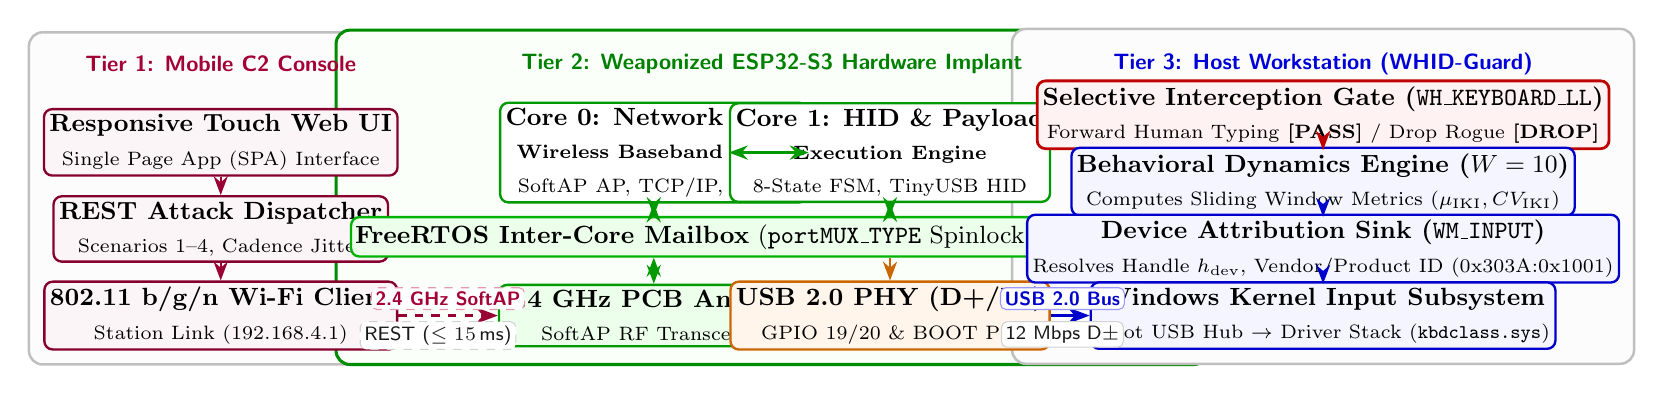
\begin{tikzpicture}[
    >=Stealth,
    font=\small,
    % Outer Container Styles
    tier_box/.style={
        rectangle,
        rounded corners=5pt,
        draw=gray!50,
        line width=0.9pt,
        fill=gray!2,
        inner sep=5pt
    },
    % Module Card Styles
    c2_card/.style={
        rectangle,
        rounded corners=3pt,
        draw=purple!70!black,
        line width=0.85pt,
        fill=purple!4!white,
        minimum width=3.8cm,
        minimum height=0.62cm,
        inner sep=2pt,
        align=center
    },
    soc_chip/.style={
        rectangle,
        rounded corners=5pt,
        draw=green!55!black,
        line width=1.1pt,
        fill=green!2!white,
        inner sep=5pt
    },
    core_box/.style={
        rectangle,
        rounded corners=3pt,
        draw=green!60!black,
        line width=0.85pt,
        fill=white,
        minimum width=2.45cm,
        minimum height=1.05cm,
        inner sep=2pt,
        align=center
    },
    ipc_box/.style={
        rectangle,
        rounded corners=3pt,
        draw=green!70!black,
        line width=0.85pt,
        fill=green!8!white,
        minimum width=5.4cm,
        minimum height=0.50cm,
        inner sep=1.5pt,
        align=center
    },
    hw_box/.style={
        rectangle,
        rounded corners=3pt,
        draw=orange!80!black,
        line width=0.85pt,
        fill=orange!8!white,
        minimum width=2.45cm,
        minimum height=0.62cm,
        inner sep=2pt,
        align=center
    },
    host_card/.style={
        rectangle,
        rounded corners=3pt,
        draw=blue!80!black,
        line width=0.85pt,
        fill=blue!4!white,
        minimum width=4.5cm,
        minimum height=0.52cm,
        inner sep=2pt,
        align=center
    },
    gate_card/.style={
        rectangle,
        rounded corners=3pt,
        draw=red!75!black,
        line width=1.0pt,
        fill=red!5!white,
        minimum width=4.5cm,
        minimum height=0.52cm,
        inner sep=2pt,
        align=center
    },
    % Badges
    lbl/.style={
        font=\sffamily\scriptsize,
        fill=white,
        draw=gray!35,
        line width=0.4pt,
        rounded corners=2pt,
        inner sep=1.5pt,
        align=center,
        text=black!90
    },
    lbl_purple/.style={
        font=\sffamily\scriptsize\bfseries,
        fill=white,
        draw=purple!40,
        line width=0.4pt,
        rounded corners=2pt,
        inner sep=1.5pt,
        align=center,
        text=purple!85!black
    },
    lbl_green/.style={
        font=\sffamily\scriptsize\bfseries,
        fill=white,
        draw=green!50!black,
        line width=0.4pt,
        rounded corners=2pt,
        inner sep=1.5pt,
        align=center,
        text=green!60!black
    },
    lbl_blue/.style={
        font=\sffamily\scriptsize\bfseries,
        fill=white,
        draw=blue!40,
        line width=0.4pt,
        rounded corners=2pt,
        inner sep=1.5pt,
        align=center,
        text=blue!80!black
    }
]

% ==============================================================================
% TIER 1: Out-of-Band Wireless Mobile Controller (C2) (Center x = 2.0)
% ==============================================================================
\node[font=\sffamily\bfseries\footnotesize, text=purple!85!black] (t1_title) at (2.0, 1.95) {Tier 1: Mobile C2 Console};

\node[c2_card] (c2_web)  at (2.0, 0.95) {\textbf{Responsive Touch Web UI}\\[1pt]\scriptsize Single Page App (SPA) Interface};

\node[c2_card] (c2_api)  at (2.0, -0.15) {\textbf{REST Attack Dispatcher}\\[1pt]\scriptsize Scenarios 1--4, Cadence Jitter};

\node[c2_card] (c2_wifi) at (2.0, -1.25) {\textbf{802.11 b/g/n Wi-Fi Client}\\[1pt]\scriptsize Station Link ($192.168.4.1$)};

\draw[->, line width=0.85pt, draw=purple!80!black] (c2_web.south) -- (c2_api.north);
\draw[->, line width=0.85pt, draw=purple!80!black] (c2_api.south) -- (c2_wifi.north);

\begin{scope}[on background layer]
    \node[tier_box, fit=(t1_title) (c2_web) (c2_api) (c2_wifi)] (tier1_bg) {};
\end{scope}

% ==============================================================================
% TIER 2: Embedded ESP32-S3 Hardware Implant (Center x = 9.0)
% ==============================================================================
\node[font=\sffamily\bfseries\footnotesize, text=green!50!black] (t2_title) at (9.0, 1.95) {Tier 2: Weaponized ESP32-S3 Hardware Implant};

% Core 0 Box (Left, x = 7.5, y = 0.82)
\node[core_box] (core0) at (7.5, 0.82) {
    \textbf{Core 0: Network \& C2}\\[1pt]
    \scriptsize\textbf{Wireless Baseband Stack}\\[1pt]
    \scriptsize SoftAP AP, TCP/IP, REST
};

% Core 1 Box (Right, x = 10.5, y = 0.82)
\node[core_box] (core1) at (10.5, 0.82) {
    \textbf{Core 1: HID \& Payload}\\[1pt]
    \scriptsize\textbf{Execution Engine}\\[1pt]
    \scriptsize 8-State FSM, TinyUSB HID
};

% Spinlock communication between cores (Clean bidirectional arrow)
\draw[<->, line width=0.85pt, draw=green!60!black] (core0.east) -- (core1.west);

% Spinlock Shared Mailbox (Center x = 9.0, y = -0.25)
\node[ipc_box] (ipc) at (9.0, -0.25) {
    \textbf{FreeRTOS Inter-Core Mailbox} (\texttt{portMUX\_TYPE} Spinlock, Ring Buffer)
};

\draw[<->, line width=0.85pt, draw=green!60!black] (core0.south) -- (core0.south |- ipc.north);
\draw[<->, line width=0.85pt, draw=green!60!black] (core1.south) -- (core1.south |- ipc.north);

% Hardware Peripherals (Bottom, y = -1.25)
\node[hw_box, draw=green!60!black, fill=green!8!white] (ant_hw) at (7.5, -1.25) {
    \textbf{2.4 GHz PCB Antenna}\\[1pt]\scriptsize SoftAP RF Transceiver
};

\node[hw_box] (usb_hw) at (10.5, -1.25) {
    \textbf{USB 2.0 PHY (D+/D-)}\\[1pt]\scriptsize GPIO 19/20 \& BOOT Pin
};

\draw[<->, line width=0.85pt, draw=green!60!black] (ant_hw.north) -- (ant_hw.north |- ipc.south);
\draw[->, line width=0.85pt, draw=orange!80!black] (ipc.south -| usb_hw.north) -- (usb_hw.north);

\begin{scope}[on background layer]
    \node[soc_chip, fit=(t2_title) (core0) (core1) (ipc) (ant_hw) (usb_hw)] (soc_bg) {};
\end{scope}

% ==============================================================================
% TIER 3: Host Workstation & WHID-Guard Defense (Center x = 16.0)
% ==============================================================================
\node[font=\sffamily\bfseries\footnotesize, text=blue!85!black] (t3_title) at (16.0, 1.95) {Tier 3: Host Workstation (WHID-Guard)};

\node[gate_card] (host_gate) at (16.0, 1.30) {
    \textbf{Selective Interception Gate (\texttt{WH\_KEYBOARD\_LL})}\\[1pt]
    \scriptsize Forward Human Typing \textbf{[PASS]} / Drop Rogue \textbf{[DROP]}
};

\node[host_card] (host_engine) at (16.0, 0.45) {
    \textbf{Behavioral Dynamics Engine ($W=10$)}\\[1pt]
    \scriptsize Computes Sliding Window Metrics ($\mu_{\text{IKI}}, CV_{\text{IKI}}$)
};

\node[host_card] (host_raw) at (16.0, -0.40) {
    \textbf{Device Attribution Sink (\texttt{WM\_INPUT})}\\[1pt]
    \scriptsize Resolves Handle $h_{\text{dev}}$, Vendor/Product ID (0x303A:0x1001)
};

\node[host_card] (host_kernel) at (16.0, -1.25) {
    \textbf{Windows Kernel Input Subsystem}\\[1pt]
    \scriptsize Root USB Hub $\rightarrow$ Driver Stack (\texttt{kbdclass.sys})
};

% Ascending defense pipeline inside Tier 3
\draw[->, line width=0.85pt, draw=blue!80!black] (host_kernel.north) -- (host_raw.south);
\draw[->, line width=0.85pt, draw=blue!80!black] (host_raw.north) -- (host_engine.south);
\draw[->, line width=0.9pt, draw=red!75!black] (host_engine.north) -- (host_gate.south);

\begin{scope}[on background layer]
    \node[tier_box, fit=(t3_title) (host_gate) (host_engine) (host_raw) (host_kernel)] (tier3_bg) {};
\end{scope}

% ==============================================================================
% INTER-TIER CONNECTIONS (Clean, Straight Horizontal Flows at y = -1.25!)
% ==============================================================================
% Tier 1 (Wi-Fi) -> Tier 2 (PCB Antenna) at y = -1.25
\draw[->, line width=1.1pt, draw=purple!80!black, dashed] (c2_wifi.east) -- (ant_hw.west)
    node[pos=0.5, above=2pt, lbl_purple] {2.4 GHz SoftAP}
    node[pos=0.40, below=2pt, lbl] {REST ($\le 15$\,ms)};

% Tier 2 (USB 2.0 PHY) -> Tier 3 (Kernel / USB Hub) at y = -1.25
\draw[->, line width=1.1pt, draw=blue!80!black] (usb_hw.east) -- (host_kernel.west)
    node[pos=0.30, above=2pt, lbl_blue] {USB 2.0 Bus}
    node[pos=0.30, below=2pt, lbl] {12 Mbps D$\pm$};

\end{tikzpicture}
\end{document}
